\chapter{3D Phase Tracking Monte Carlo Algorithm}\label{sec:phase}

\section{Introduction}\label{sec:besintro}

%Intro = mention complex beams and their uses then move onto gaussian and bessel beams

Bessel beams have been the subject of intense research since their discovery in 1987~\cite{durnin1987diffraction,durnin1987exact}. Durnin noticed that the blah blah.
%Bessel beams have since been used for blah blah
%They are really good and like are better than Gaussian beams allegedly.

This chapter examines how Bessel beams compare to other beam in a scattering medium. 
We investigate if the Bessel beams self-healing property has any effect in a turbid medium.
We examine Bessel beams and the other beams by creating a novel~\gls*{mcrt} algorithm that allows the tracking of a photon as it propagates through a medium. 
The main focus of this chapter, is validation of our new novel technique, followed by using the new algorithm ($\varphi MC$) to compare Gaussian and Bessel beams, to see which one preforms better in a turbid medium. 
This chapter also extends out novel algorithm to other complex, diffraction less beams


%motivation = better imaging of chick embryos etc


\section{Theory}\label{sec:bestheory}

The \gls*{mcrt} algorithm as described in~\cref{sec:mcrt}, must be adjusted so that wave phenomena such as interference and diffraction can be modelled. 
Modelling these wave behaviours allows us to model complex beams, where these phenomena are required to form the beam, e.g Bessel beams. 
As \gls*{mcrt} is a ballistic simulation of photon packets, meaning that the \gls*{mcrt} simulation presented thus far in this thesis only modelled the ballistic behaviour of photons. 
However for the work presented in this chapter, wave like behaviour is crucial to modelling the various experiments and phenomena.

To convert a ballistic simulation of photon packets into a ballistic/wave-like simulation, the complex phase of each photon packet is tracked.
This is achieved, by simply tracking the complex phase of the photon as it propagates through a medium.
~\Cref{eqn:phase} shows how the phase is calculated.

\begin{equation}
    \varphi = cos\left(\frac{2 \pi l}{\lambda}\right) + i\ sin\left(\frac{2 \pi l}{\lambda}\right)
    \label{eqn:phase}
\end{equation}

Where $\varphi~[-]$ is the phase of a photon packet, $l\ [m]$ is the distance the photons has travelled, and $\lambda~[m]$ is the wavelength of the photon.
Now we can calculate the phase of a photon at a position $P_o$, if we know the distance it has travelled, and its original phase,~\cref{fig:phase-diag}.

\begin{figure}[!ht]
    \centering
    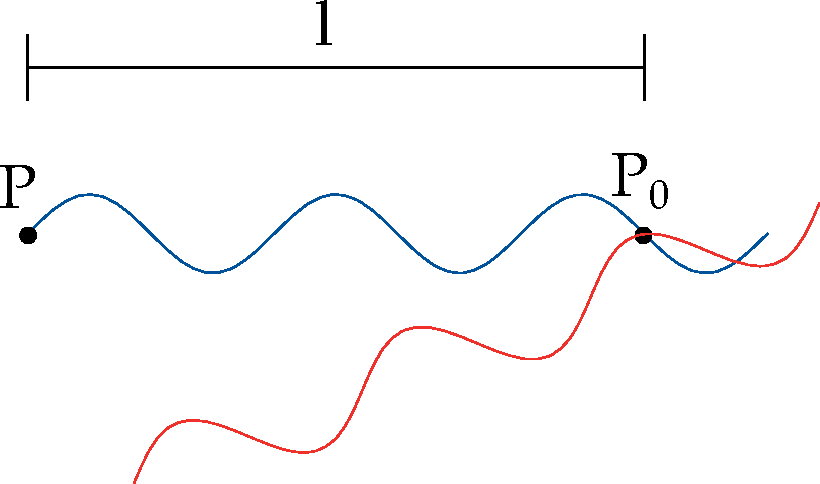
\includegraphics[width=0.5\textwidth]{phase-diag.pdf}
    \caption{Example of phase calculation when a photon has travelled a distance l. Figure also show an example of interference between two photons.}
    \label{fig:phase-diag}
\end{figure}

To be able model the wave-like behaviour of photons, we let the photons packets interfere with one another in a volume or area element. 
We do not model the interference at a point in space where photons packets cross one another as due to the ballistic nature of the \gls*{mcrt} simulation, this does not occur with enough frequency in order to give a good signal to noise ratio. 
Thus, interference takes place in a volume, $dV$, or area element, $dA$, instead.
To calculate the interference from the phase, the phase is summed in each volume or area element and the absolute value taken, and then squared.~\Cref{eqn:intense} shows the equation for interference for a volume element $dV$. A similar relation for calculating the interference on an area element $dA$ also exists.

\begin{equation}
I(\xi)=\left| \sum\limits_{\xi}cos\left(\frac{2\pi l}{\lambda}\right) + i \sum\limits_{\xi}sin\left(\frac{2\pi l}{\lambda}\right)\right|^2,\ \ \ \xi=(x,y,z)
\label{eqn:intense}
\end{equation}

\noindent Where:

\indent $l$ is the total distance travelled by a photon [$m$];

\indent $\lambda$ is the wavelength of the photon [$m$];

\indent $I$ is the intensity at the $\xi^{th}$ cell [$W m^{-2}$];

\indent and $\xi$ is the $x^{th}$, $y^{th}$, $z^{th}$ cell, volume $dV$.

\medskip

As the \gls*{mcrt} simulation is now a quasi ballistic/wave simulation of photon behaviour, comparisons between the simulations and, theoretical and experimental data to prove this model is accurate. However before validation of the model takes place, one further principle needs to be introduced that is required for our model to work.

\subsection{Huygens-Fresnel Principle}

The Huygens-Fresnel principle is a method that is used to help model the propagation of waves in the far field limit and the near field limit. 

The Huygens principle states: 

\medskip

``Every point on a wavefront acts as a source of spherical wavelets, and that the sum of all the wavelets forms the wavefront.''***ref***

\medskip

The principle is illustrated in~\cref{fig:huygensillis}. Christiaan Huygens postulated this principle in 1678.
The principle allowed Huygens to derive laws of refraction and reflection using this principle, but it failed to describe diffraction effects.
This led to Augustin-Jean Fresnel in 1818, combining the Huygens principle with his own theory of interference.
This principle, the Huygens-Fresnel principle, gave an accurate description of the propagation of light and diffraction effects.
This was achieved by allowing the secondary wavelets to self interfere with one another, giving rise to an accurate description of the physical phenomena.
Later, Gustav Kirchhoff gave a rigours mathematical description of the Huygens-Fresnel principle, which is the basis of diffraction theory. *refs for this section*

Our algorithm uses the Huygens-Fresnel principle to simulate diffraction effects, that would otherwise be absent from the simulation.
The Huygens-Fresnel principle is implemented by sampling the light source on the surface of any lens or in a slit.




%allows us to calculate complex amplitude at a given point. 
%inclination factor no backward waves.
%used in diffraction theory -> kirchoffs
%
%fresnel and fraunhoefer diffraction -> validation of algorithm
%fresnel close
%fraunhoefer far away

\begin{figure}[!ht]
    \centering
    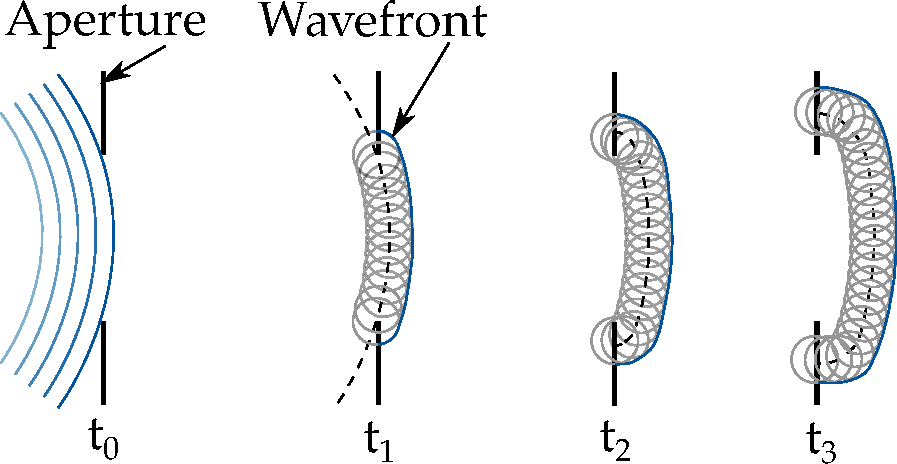
\includegraphics[width=0.7\textwidth]{huygens.pdf}
    \caption{Illustration of the Huygens-Fresnel principle. At $t_0$ a wave is incident on an aperture. Times $t_1,\ t_2,\ \text{and}\ t_3$ show the evolution of the wavefront using the Huygens-Fresnel principle.}
    \label{fig:huygensillis}
\end{figure}

\subsection{Validation of Phase Tracking Algorithm}

\subsubsection*{Double Slit Experiment}

The first test of our phase tracking algorithm, is to compare our simulation to a double slit experiment.
The double slit experiment, is a simple experiment where monochromatic plane wave of light is incidence on two slits distance apart $a$, and width $b$, and the interference pattern is observed on a screen a distance $d$ away from the slits.

%In this experiment blah bla ***

\begin{equation}
    I(\theta) \propto cos^2\left(\frac{\pi d\ sin \theta}{\lambda}\right)sinc^2\left(\frac{\pi b\ sin\theta}{\lambda}\right)
\end{equation}

Where the $sinc$ function is defined as $\tfrac{sin(x)}{x}$, for $x\ \neq 0$, d is the slit separation and $\theta$ is the angular spacing of the fringes.


\begin{figure}[!ht]
    \centering
    % \includegraphics[]{}
    \caption{Comparison of theory and simulation for the double slit experiment. $\lambda$ is $x nm$, $b$ is, and $d$}
    \label{fig:doubleslitcomp}
\end{figure}

\subsubsection*{Diffraction by a Square Slit}
$\varphi MC$ is also validated by simulating diffraction from a square aperture in the far and near field.

%near field == fresnel
%far field == fraunhoefer

In the Fresnel regime, the electric field at a point p is

\begin{equation}
\hat{E}_p=\frac{\varepsilon_0}{2(\rho_0+r_0)}e^{i[k(\rho_0+r_0)-\omega t]}\int^{u_2}_{u_1} e^{i\pi u^2/2}du \int^{v_2}_{v_1} e^{i\pi v^2/2}dv
\label{eqn:fresEfield}
\end{equation}

Where $k$ is a wavevector, $\varepsilon_0$ is permittivity of free space, and the other symbols have their meanings as in~\cref{fig:aperture}. \textit{u} and \textit{v} are the following dimensionless variables:

\begin{align}
u&=y\sqrt{\frac{2(\rho_0+r_0)}{\lambda\rho_0r_0}}\\
v&=z\sqrt{\frac{2(\rho_0+r_0)}{\lambda\rho_0r_0}}
\end{align}


Where $(y,z)$ are the coordinates of the point $a$ in~\cref{fig:aperture}.
\medskip

Using~\cref{eqn:fresneleqn}, where $C(w)$ and $S(w)$ are the Fresnel integrals as in~\cref{eqn:fresint1,eqn:fresint2},~\cref{eqn:fresEfield} can then be transformed into an intensity, by taking the absolute value and squaring, yielding~\cref{eqn:fresIntensityp}:

\begin{equation}
\int_{w}^{w'}e^{i\pi u^2/2}du=C(w)+iS(w)
\label{eqn:fresneleqn}
\end{equation}


\begin{align}
S(w)&=\int^w_0 sin\left(\frac{\pi w'^2}{2}\right)dw'\label{eqn:fresint1}\\
C(w)&=\int^w_0 cos\left(\frac{\pi w'^2}{2}\right)dw'\label{eqn:fresint2}
\end{align}


\begin{equation}
I_p = \frac{I_u}{4} \{[C(u_2) - C(u1)]^2 + [S(u_2) - S(u_1)]^2\} \times \{[C(v_2) - C(v_1)]^2 + [S(v_2) - S(v_1)]^2\}
\label{eqn:fresIntensityp}
\end{equation}

\Cref{eqn:fresIntensityp} gives the intensity of the field at the point $p$, on axis for a square aperture. In order to calculate the intensity of the axis around the point $p$,~\cref{eqn:fresIntensityp} is used, but the $y$ and $z$ variables are perturbed in the desired direction to yields the intensity at the point $p+d$, where d is the distance the aperture is perturbed.

\begin{figure}[!ht]
    \centering
    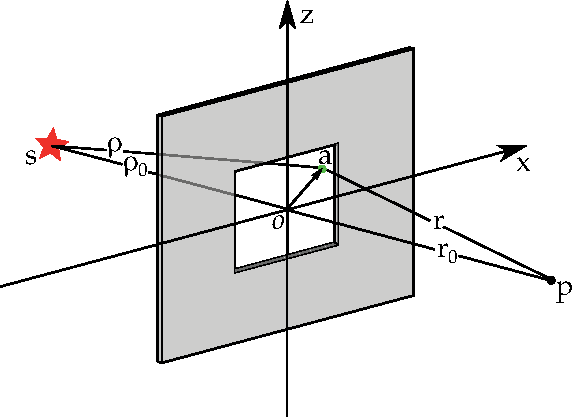
\includegraphics[width=0.75\textwidth]{aperture.pdf}
    \caption{Fresnel diffraction at a square aperture.}
    \label{fig:aperture}
\end{figure}


\begin{equation}
F = a\sqrt{\frac{2}{\lambda r_0}}
\label{eqn:fnumber}
\end{equation}

In $\varphi MC$, the above experiment is simulated. A square slit is uniformly sampled in the $y$, and $z$. A random direction is then sampled, ensuring that the direction points towards the detector screen.

The detector screen's distance from the aperture is then varied and the intensity on the screen is measured for $10^{10}$ photons released from the aperture, as Huygens wavelets.

\FloatBarrier

\section{Bessel Beams}

The first ``complex'' beam simulated using $\varphi MC$ is a Bessel beam. 
Bessel beams are non-diffractive solutions to the wave equation. 
Bessel beams were first shown to blah


% *** Bessel beams non diffracting
%     but are they - some debate over this
%     self reconstructing
%     central core does not diffract like Gaussian
%     quasi Bessel beam -> infinite rings not possible -> infinite energy
%     Bessel beam theory form of equation -> intensity
%     pics of Bessel beam + higher orders
%     geometry of Bessel beams
%     Bessel beams in code
%     results
% ***


\begin{figure}[!ht]
    \centering
    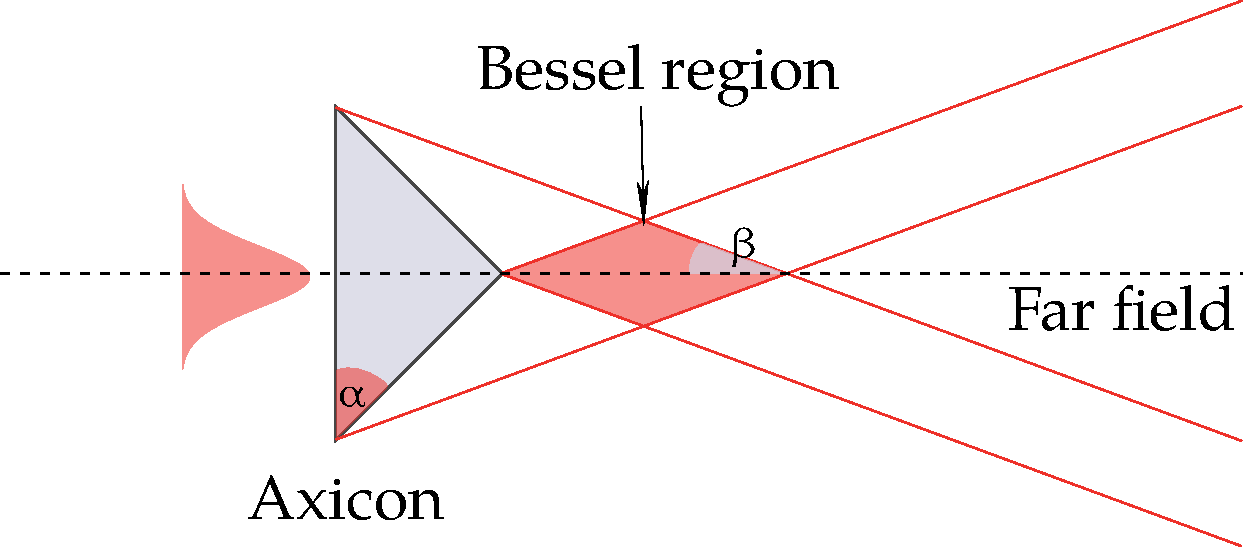
\includegraphics[width=0.6\textwidth]{bessel.pdf}
    \caption{Geometry of a Bessel beam, generated by an axicon lens. $\beta$ is the angle with the optical axis, and the angle of the conical waves. $\alpha$ is the axicon angle.}
    \label{fig:besselgeo}
\end{figure}

From the scalar description of the electric component of the beam, we get:

\begin{equation}
    E(r,z)=E_0\sqrt{\frac{2\pi k z w_0sin(\beta)}{z_{max}}}\ \text{exp}^{\left(-\frac{z^2}{z_{max}^2}-\frac{i\pi}{4}\right)}\ J_0\left(krsin(\beta)\right)\ \text{exp}^{\left(ikzcos(\beta)\right)}
    \label{eqn:besselEfield}
\end{equation}

\noindent Where:

    \indent k is the wavevector, $k=\tfrac{2\pi}{\lambda}$ [$m$];

    \indent z is the distance from the axicon tip [$m$]; 

    \indent $\beta$ is the angle the wavefront propagates at (see~\cref{fig:besselgeo}) [$rad$]; 

    \indent $w_0$ is the $\tfrac{1}{e^2}$ width of the input Gaussian beam [$m$]; 

    \indent $J_0$ is the Bessel function of the first order; 

    \indent r is radial distance from the optical axis [$m$]. 

\medskip


~\Cref{eqn:besselEfield} gives the electric field for a Bessel beam. The intensity can be calculated using:

\begin{equation}
    I(r,z)=\frac{c\epsilon_0\left|E_0\right|^2}{2}
    \label{eqn:besselintsub}
\end{equation}

Using the definition total power transmitted by a beam as:

\begin{equation}
    P=\frac{\pi I_0w_0^2}{2}
    \label{eqn:pwrdef}
\end{equation}

Where $I_0$ is defined as on axis intensity of the incident Gaussian beam.

\begin{equation}
    I_0=\frac{c\epsilon_0E_0^2}{2}
    \label{eqn:intdef}
\end{equation}

Substituting~\cref{eqn:besselEfield,eqn:intdef,eqn:pwrdef} into~\cref{eqn:besselintsub} yields:

\begin{equation}
    I(r,z)=\frac{4k_rP}{w_0}\frac{z}{z_{max}}J_0^2\left(k_r\ r\right)\text{exp}^{\left(-\frac{2z^2}{z^2_{max}}\right)}
    \label{eqn:besselInt}
\end{equation}


\noindent Where:

    \indent $k_r$ is the radial wavevector, $k_r=k sin(\beta)$;

    \indent P is the power of the incident Gaussian beam.

    \medskip

To check out method accurately models Bessel beams, we compare out beam to theoretical expressions and experimental data.

To compare against a theoretical Bessel beam, a Bessel beam is modelled in the MCRT phase simulation, and propagated through air past the ``Bessel region''. 
A slice of the intensity is then plotted against what the theory predicts the Bessel beam should look like. 
A check of how the Bessel beam propagates in the far field is also preformed.


~\Cref{eqn:besselInt} gives the profile of a theoretical Bessel beam at a depth $z_{max}$, this is plotted against the simulation when $\tfrac{4k_rPz}{w_0z_{max}}e^{-2\left(\tfrac{z}{z_{max}}\right)^2}=1$, with the simulation similarly normalised, by normalising to the maximum intensity of the image generated. ~\Cref{fig:besselCompare} shows this comparison.


\begin{figure}[!ht]
    \centering
    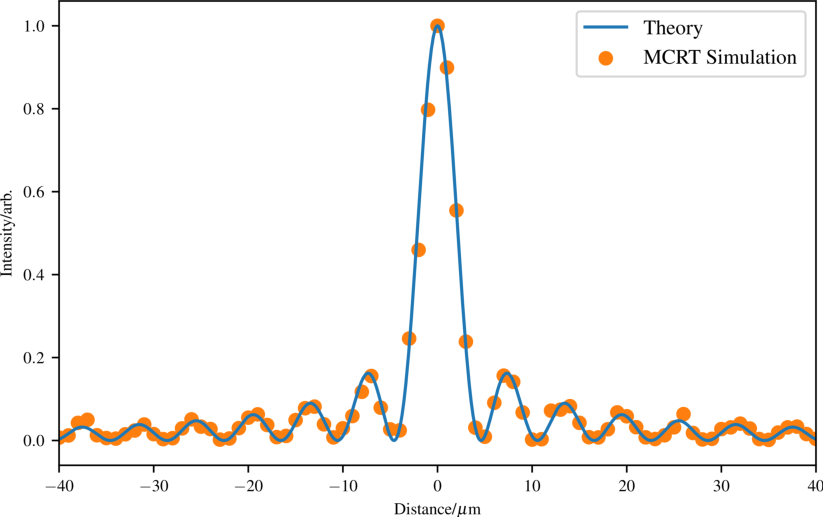
\includegraphics[width=0.95\textwidth]{compare-theory.pdf}
    \caption{Comparison of theoretical and MCRT simulation of a Bessel beams, with intensity normalised. The results from $\varphi MC$ show good agreement with the theory.}
    \label{fig:besselCompare}
\end{figure}

To ensure our algorithm works in turbid media, we carried out an experiment where a Bessel beam was propagated through a medium of varying turbidity.
A laser, wavelength $488~nm$, with a Gaussian profile is shone on an axicon lens, with angle $5~^{\circ}$.
The laser beam had a $\tfrac{1}{e^2}$ spot size of $2~mm$. 
The Bessel beam was allowed to propagate through the air for $10~cm$ before entering a cuvette of side $2~mm$.
The cuvette was filled with $500~\mu L$ of water, and various volumes of a scattering agent added.
The scattering agent used is intralipid $20~\%$ (Sigma-Aldrich), which is diluted as shown in~\cref{tab:intra}.
Dilutions of Intralipid are kept below 2\% scattering particle concentration, so that the scattering exhibited by the intralipid is in the independent scattering regime.
This allows the linear scaling of the optical properties by concentrations~\cite{aernouts2013supercontinuum,vardaki2015studying,di2011effect}.
Images of the Bessel beam as it emerges from the cuvette are taken for comparison with out algorithm.
~\Cref{fig:expsetup} shows the experimental setup.

\begin{figure}[ht!]
    \centering
    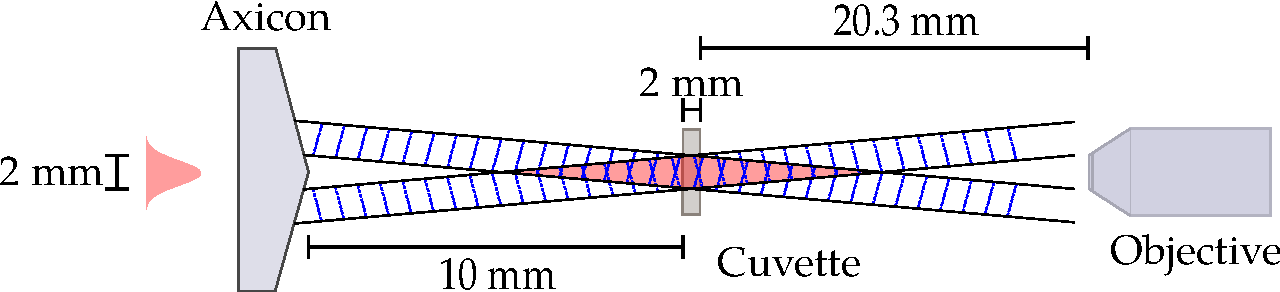
\includegraphics[width=0.8\textwidth]{bessel-exp-setup.pdf}
    \caption{Experimental setup for propagating a Bessel beam through a cuvette filled with varying concentrations of Intralipid 20\%. Bessel beam is imaged by an $20\times$ objective lens and a Grasshopper 3 camera.}
    \label{fig:expsetup}
\end{figure}

\begin{table}[!ht]
\centering
    \begin{tabular}{cc|cc}
        \hline
        \multicolumn{2}{c|}{Volume/$\mu L$} & \multicolumn{2}{|c}{Intralipid concentration}                       \\
        Intralipid                & $H_2O$  & Volume/\%      & Scattering particle/\% \\ \hline
        \multicolumn{1}{c|}{0}    & 500     & \multicolumn{1}{c|}{0.0}       & 0.0                                    \\
        \multicolumn{1}{c|}{2}    & 500     & \multicolumn{1}{c|}{0.39841} & 0.0908                                \\
        \multicolumn{1}{c|}{4}    & 500     & \multicolumn{1}{c|}{0.79365} & 0.1816                                \\
        \multicolumn{1}{c|}{6}    & 500     & \multicolumn{1}{c|}{1.18577} & 0.2724                                \\
        \multicolumn{1}{c|}{8}    & 500     & \multicolumn{1}{c|}{1.57480} & 0.3632                                \\
        \multicolumn{1}{c|}{10}   & 500     & \multicolumn{1}{c|}{1.96078} & 0.4534                                \\
        \multicolumn{1}{c|}{12}   & 500     & \multicolumn{1}{c|}{2.34375} & 0.5448                                \\ \hline
    \end{tabular}
    \caption{Intralipid solutions used for experiment.}
    \label{tab:intra}
\end{table}


To model within $\varphi MC$, the experimental setup we simplify the setup considerably.
The simulation models the propagation of a photon packet through the axicon to its conical surface. 
On the conical surface the Huygens-Fresnel principle is invoked, and the packet is sampled onto the surface of the medium (cuvette).
The sampling of the photon onto the surface of the medium, speeds the algorithm up, as it does not need to simulate the photons that would ``miss'' the medium.
From there the usual~\gls*{mcrt} method propagates the packet through the medium while tracking its phase, and scattering the packet until it leaves the medium.
If the packet leaves the medium to any side other than the far side of the cuvette (e.g any side of the cuvette not facing the objective lens), then it is discarded.
If the packet leaves the medium on the objective lens facing side, then the packet is recorded by its phase onto an area element.
For each intralipid concentration $3.2\times10^{11}$ photons are run over 32 cores, taking $\sim 4$ hours for the 0.5448\% intralipid concentration.
Once all the photon packets have been run, the image is the phase is converted into intensity, as in~\cref{eqn:intense}, but in 2D.

\Cref{fig:compareexpbessel} shows the results from the experiment and simulation. The simulation shows good agreement with experimental data.

\begin{figure}[!ht]
\centering
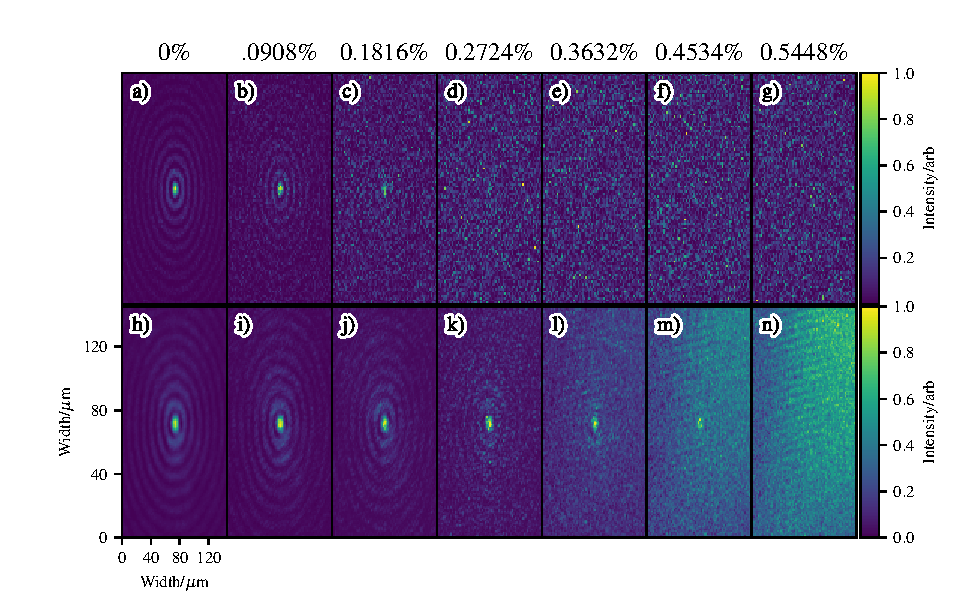
\includegraphics[width=0.95\textwidth]{compare-exp.pdf}
\caption{Comparison of experimental and simulation data for propagation of a Bessel beam produced by an axicon, through mediums of various turbidity. Images a) to g) is the data from $\varphi MC$, and h) to n) are the experimental data. Concentrations along the top are the concentration of scattering particles in each solution as in~\cref{tab:intra}. All images cropped so they are the same size.}
\label{fig:compareexpbessel}
\end{figure}


% \begin{figure}
% \centering
% 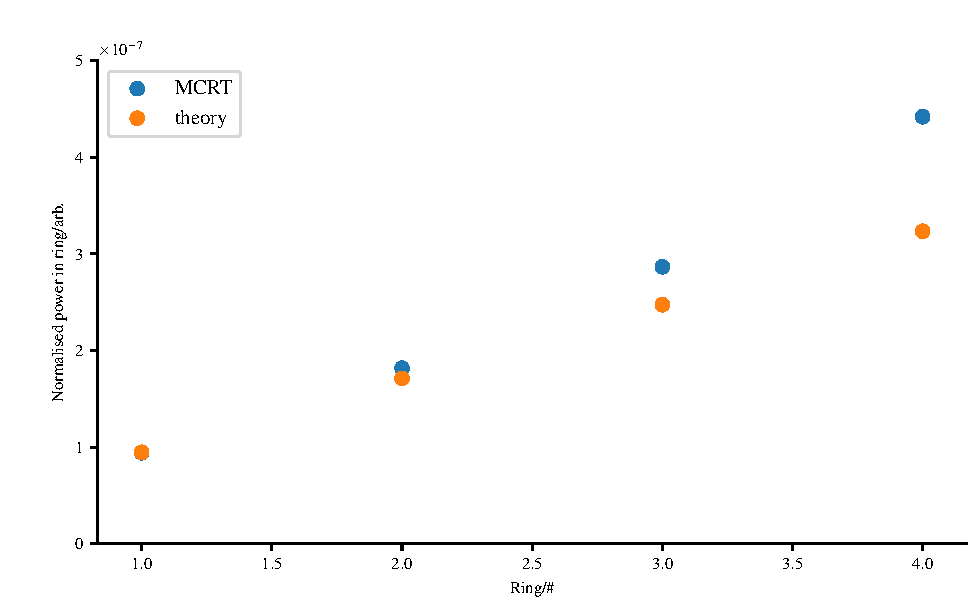
\includegraphics[scale=0.65]{pwr-rings.pdf}
% \caption{Bessel beam power in each ring.}
% \label{fig:pwrring}
% \end{figure}

% \begin{figure}
% \centering
% 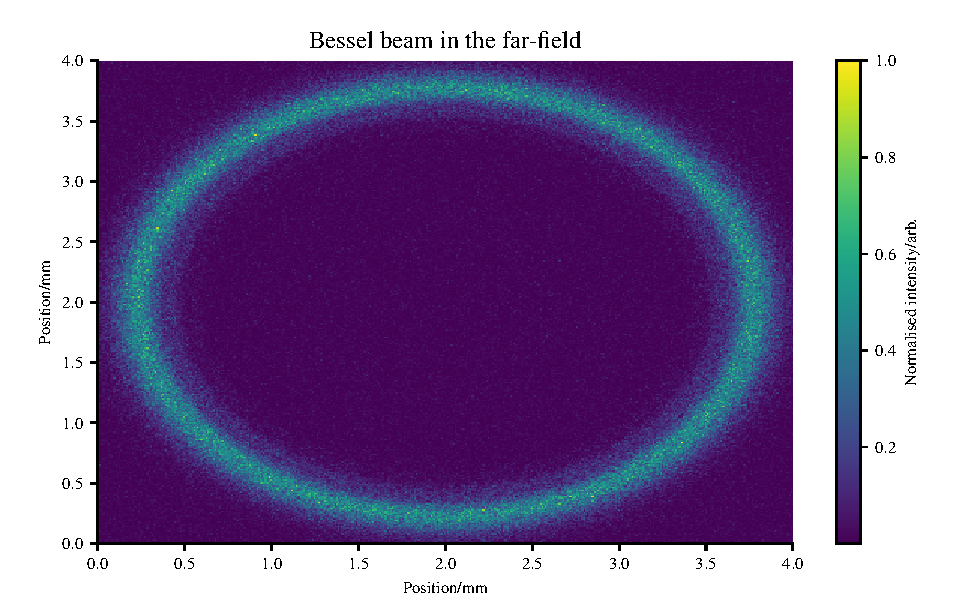
\includegraphics[width=0.95\textwidth]{far-field.pdf}
% \caption{Bessel beam in the far field.}
% \label{fig:farfield}
% \end{figure}
\FloatBarrier

\section{Gaussian Beams}

% gaussian beam theory
% geometry
% implementation of lens's -> plano-convex and aspheric
% emphasis no coding of focal distance
% spherical aberrations 
% curvature of phase change
% 
% need to find factor root 2

\section{Other Beams}

Our technique outlined in the preceding sections, can also be applied to arbitrary non-diffracting or complex beams. The only requirements for our algorithm to be able to model a complex beam, is that there is some phase delay that can be modelled analytically\footnote{It may be possible to model phase delays that are not analytical expressions. Simulating spatial light modulators may also be possible with our algorithm.}.

The first example of using our algorithm to model complex beams is to model a Laguerre-Gauss beam. A Laguerre-Gauss beam can be created by introducing a helical phase delay to a plane wave blah blah. ***put theory here + phase and interference patterns for all beams

Another example of our algorithms flexibility is that it can also model Hermite-Gauss beams, higher order Bessel beams and airy beams

\section{Comparison}

\section{Discussion}

%talk about comparison of beams. methods validity -> downside and upsides

a~\cite{mignon2016fractional}
\section{Conclusion}

%conclude shit


%sources
%cizmar thesis
%born: principles of optics
%hecht: optics
%mignon
%prahl
%fresnel/fraunhoefer paper
%thorlabs
%sacsha thesis
%kishans papers
%various axicon papers
%aspheric papers
%phase screen model
%beam steering paper
%paper that hates on mcrt
%E-field mcrt